\documentclass[
    ngerman,%globale Übergabe der Hauptsprache
%	logofile=example-image, %Falls die Logo Dateien nicht vorliegen
    authorontitle=true,
]{bfhbeamer}


%\usepackage[main=ngerman]{babel}

% Der folgende Block ist nur bei pdfTeX auf Versionen vor April 2018 notwendig
%\usepackage{iftex}
%\ifPDFTeX
%\usepackage[utf8]{inputenc}%kompatibilität mit TeX Versionen vor April 2018
%\fi


%Makros für Formatierungen der Doku
%Im Allgemeinen nicht notwendig!
%\let\code\texttt

\title{URL-Archiver - Intermediate Presentation}
\subtitle{Version 1.0}
\author[N. Dora \and A. Vejseli \and K. Wampfler]{N. Dora \and A. Vejseli \and K. Wampfler}
\institute{School of Engineering and Computer Science}
\titlegraphic*{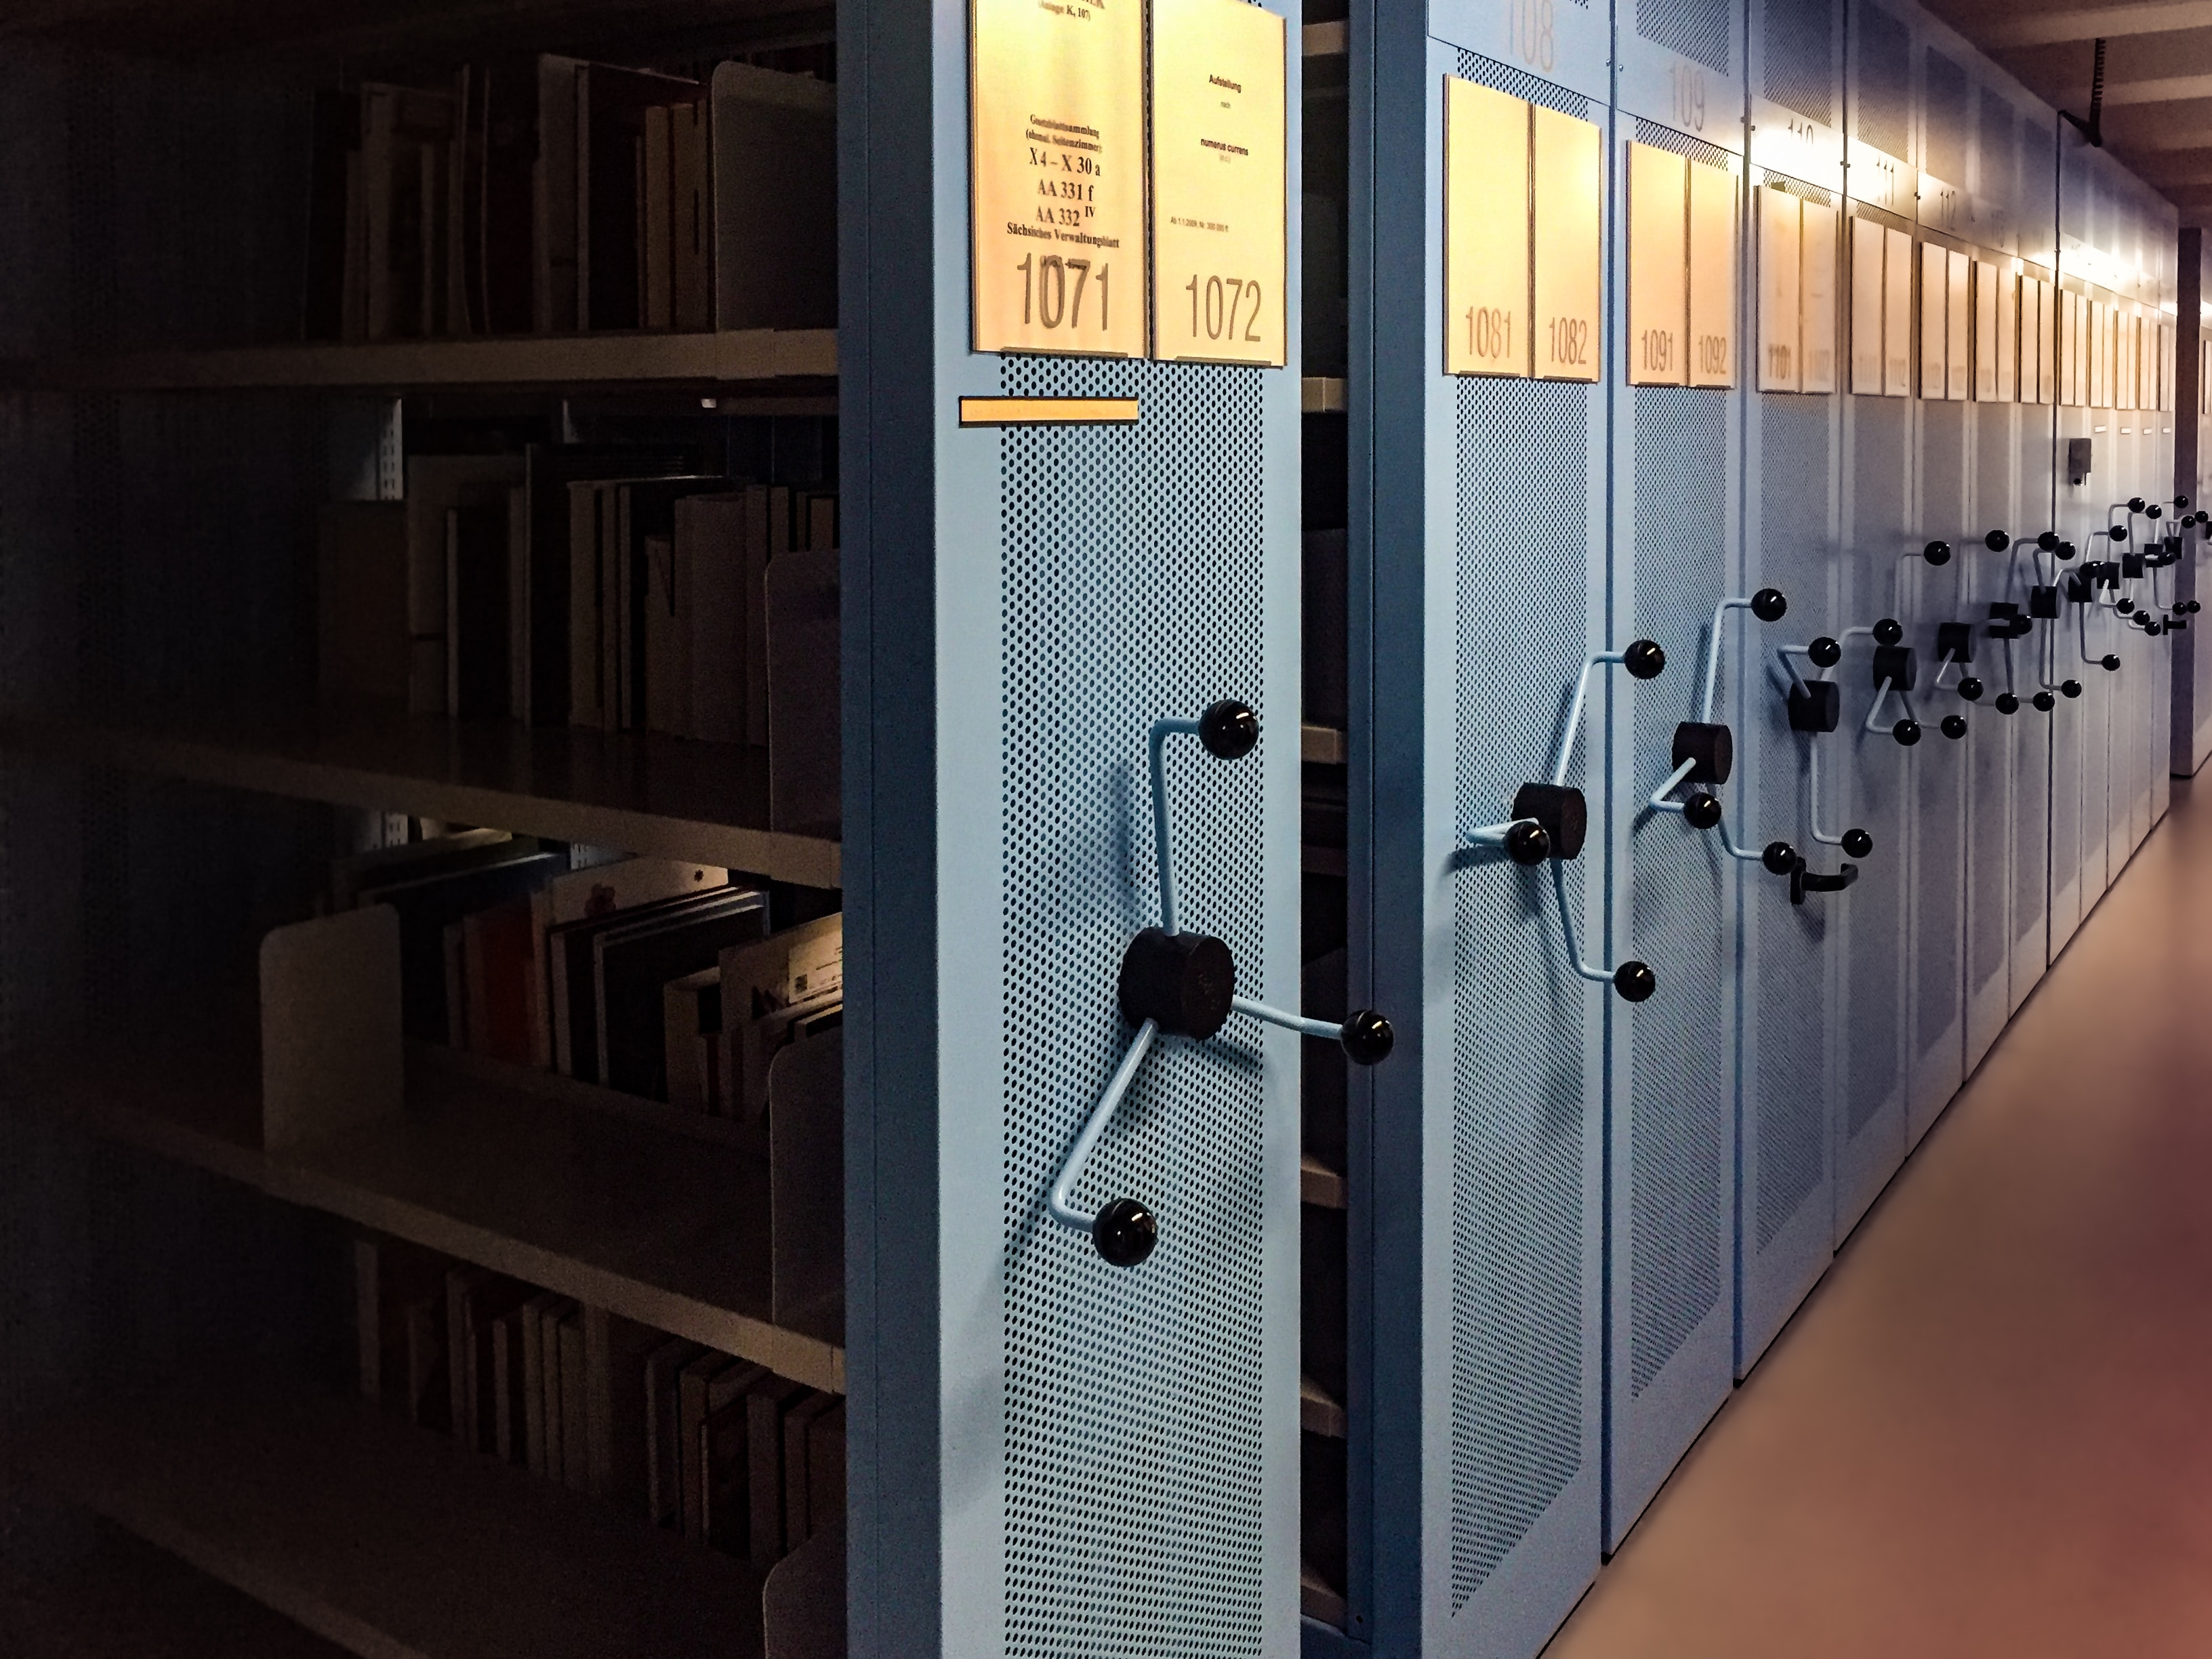
\includegraphics{pictures/archive-title-image}}%is only used with BFH-graphic and BFH-fullgraphic

%Activate the output of a frame number:
\setbeamertemplate{page number in head/foot}[framenumber]

\begin{document}

%    Was ist die Problemstellung Ihres Projektes
%   (Zielsetzungen, Anforderungen, Rahmenbedingungen)
%    Kilian
%    Wie wollen Sie die Problemstellung lösen?
%    (Architektur, Datenmodell, Prozessmodell, Technologien, usw.)
%    Nicolin
%    Wie setzen Sie das Projekt mit Scrum um?
%    Abidin Vejseli

    \setbeamertemplate{title page}[BFH-fullgraphic]
    \maketitle



    \begin{frame}{Table of Content}
        \framesubtitle{Topics Covered}
        \tableofcontents
    \end{frame}

    % Chapter one "Problem Statement"


    \section{Problem Statement}
    \setbeamertemplate{section page}[BFH-ruled]
    \frame{\sectionpage}

    \begin{frame}{Problem Statement}
        \framesubtitle{The ever changing internet}
        \begin{itemize}
            \item ever-changing internet (websites are taken down or changed)
            \item not a problem for everyday internet users but\ldots
            \item \ldots what about documents (e. g. theses, documentations etc.)
            \begin{itemize}
                \item invalid links to content-relevant information
                \item invalid quote links
                \item old documents may contain numerous broken hyperlinks
            \end{itemize}
        \end{itemize}
    \end{frame}

    \begin{frame}{Problem Statement}
        \framesubtitle{Simple Solution}
        \begin{itemize}
            \item Archive the actual state of the linked websites
            \begin{itemize}
                \item Wayback machine
                \item archive.today
                \item Memento Time Travel
                \item and many more…
            \end{itemize}
            \item But who has the time and motivation?
            \begin{itemize}
                \item \ldots to search each hyperlink
                \item \ldots to manually archive each website
            \end{itemize}
        \end{itemize}
    \end{frame}

    \begin{frame}{Objectives}
        \framesubtitle{}
        \begin{itemize}
            \item Develop a software that\ldots
            \begin{itemize}
                \item \ldots searches hyperlinks within documents
                \item \ldots is capable of archiving linked websites
                \item \ldots can store current and archived links in a file
                \item \ldots is easy and intuitive to use
            \end{itemize}
        \end{itemize}
    \end{frame}

    \begin{frame}{Requirements}
        \framesubtitle{}
        \begin{itemize}
            \item The software must be\ldots
            \begin{itemize}
                \item \ldots a Java application that is compatible with multiple platforms
                \item \ldots FLOSS-licensed
                \item \ldots capable of archiving websites on archive.ph or/and WayBackMachine
                \item \ldots capable of generating a CSV-file with key-value (URL, archived URL)
            \end{itemize}
        \end{itemize}

    \end{frame}

    \begin{frame}{General conditions}
        \framesubtitle{}
        \begin{itemize}
            \item The program code should be minimal, modular, and self-explaining
            \item The program code should be published in a git repository
            \item The project must be carried out according to scrum
            \item Public documents should be written in English
            \item LaTeX should be used for the project report
        \end{itemize}
    \end{frame}
    %-------------------------------%

    % Chapter two "Solving the Problem"


    \section{Solving The Problem}
    \setbeamertemplate{section page}[BFH-ruled]
    \frame{\sectionpage}

    \begin{frame}{Architecture}
        \framesubtitle{Employing the MVC Pattern}

        \begin{columns} % Start the columns environment
            \begin{column}{0.5\textwidth} % Define the width of the left column
                \begin{itemize}
                    \item Modular design for easy extension.
                    \item Separate data, interface, and control flow.
                    \item Facilitates the potential addition of a GUI.
                \end{itemize}
            \end{column}

            \begin{column}{0.5\textwidth} % Define the width of the right column
                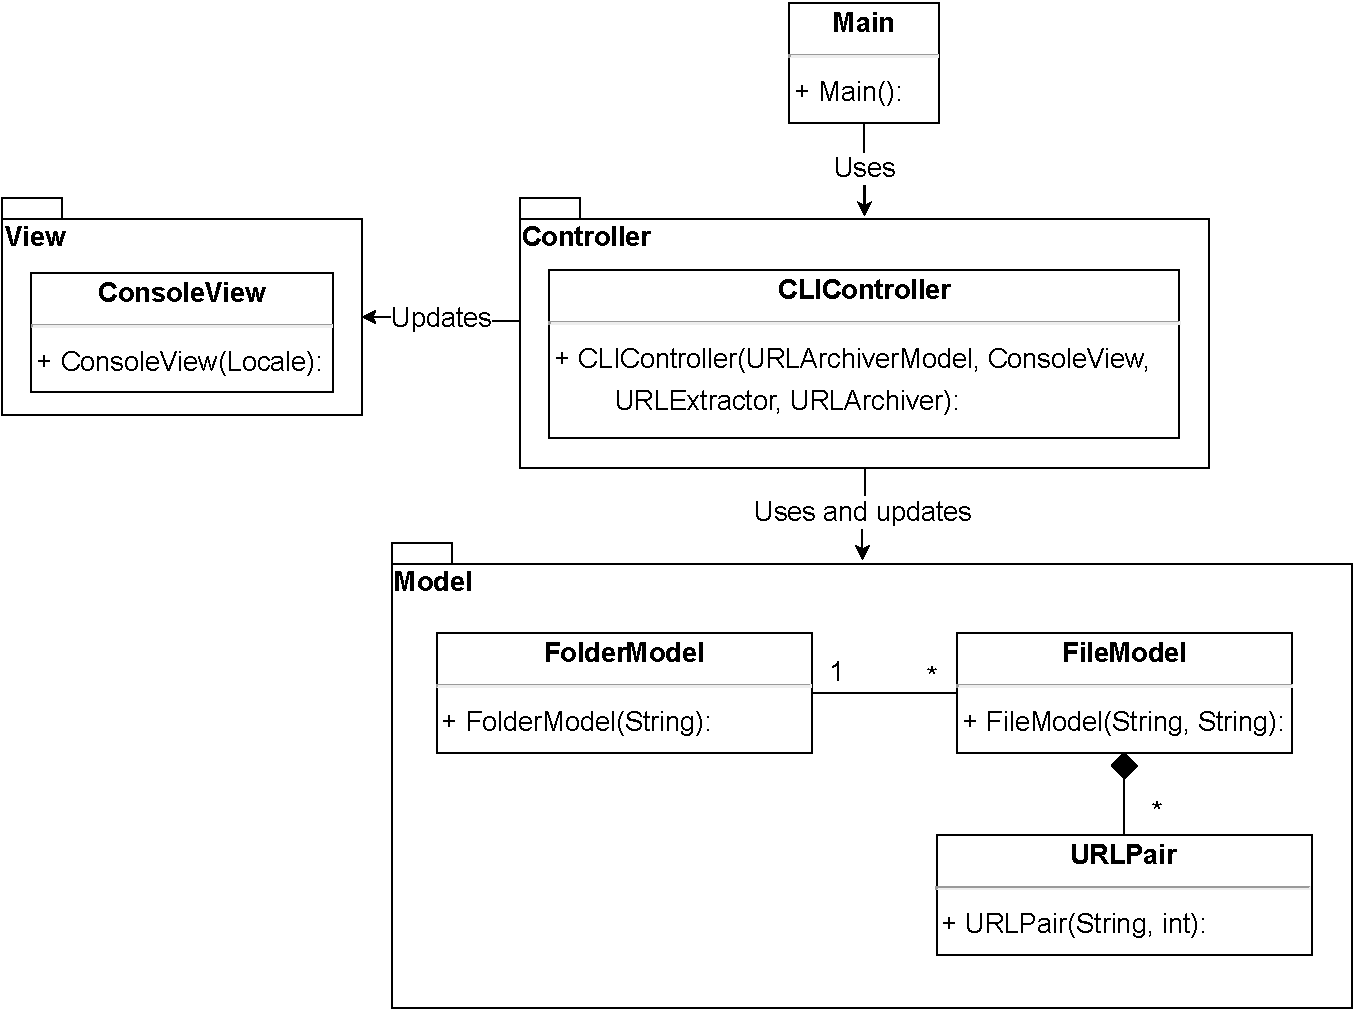
\includegraphics[width=1\textwidth]{pictures/mvc_diagram-Detailed}
            \end{column}
        \end{columns} % End the columns environment
    \end{frame}

    \begin{frame}{Architecture}
        \framesubtitle{SOLID Principles}
        \begin{itemize}
            \item Scalable and robust design.
            \item Ensures maintainability and clear code structure.
            \item Commitment to best programming practices.
        \end{itemize}
    \end{frame}

    \begin{frame}{Architecture}
        \framesubtitle{Object-Oriented Approach}
        \begin{itemize}
            \item Promotes code reusability.
            \item Logical class hierarchies.
            \item Clear relationships between modules.
        \end{itemize}
    \end{frame}

    \begin{frame}{Architecture}
        \framesubtitle{Multilanguage Support with ResourceBundle}
        \begin{itemize}
            \item Ready for global adaptability.
            \item Future-proofing architectural choice.
            \item Potential to accommodate multiple languages.
        \end{itemize}
    \end{frame}

    % Slide for Overview of the Data Model
    \begin{frame}{Overview of the Data Model}
        The data model is designed to represent and manage the data structures essential for the application's operation. It encompasses handling files, user interactions, and archiving URLs.
    \end{frame}

% Slide for Key Components
    \begin{frame}{Key Components of the Data Model}
        \begin{itemize}
            \item \textbf{FileModel}: Represents and handles individual files.
            \item \textbf{FolderModel}: Manages a collection of FileModel instances.
            \item \textbf{URLPair}: Links extracted URLs with their archived counterparts.
            \item \textbf{URLArchiverModel}: Organizes and maintains URLPairs.
            \item \textbf{UserChoice}: Enumerates possible user commands and actions.
        \end{itemize}
    \end{frame}

% Slide for Interactions and Relationships
    \begin{frame}{Interactions and Relationships}
        This model's components interact to facilitate file and URL management:
        \begin{itemize}
            \item FolderModel aggregates FileModels representing files in a folder.
            \item URLArchiverModel processes and pairs URLs from FileModels.
            \item User actions guide the flow of data through the models.
        \end{itemize}
    \end{frame}

% Slide for Use Case Flow
    \begin{frame}{Use Case Flow in the Data Model}
        A typical use case might involve:
        \begin{enumerate}
            \item A user selects an action (UserChoice).
            \item The system processes files in a folder (FolderModel with FileModels).
            \item URLs are extracted, archived, and paired (URLArchiverModel with URLPairs).
        \end{enumerate}
        This flow demonstrates the integrated operation of the data model components.
    \end{frame}

% Slide for Conclusion
    \begin{frame}{Conclusion}
        The data model is a critical framework within the application, enabling structured data manipulation, storage, and retrieval, which are fundamental to the application's functionality and user experience.
    \end{frame}


    \begin{frame}{Process model}
        \framesubtitle{Workflow for URL Extraction and Archiving}
        \begin{itemize}
            \item User can skip URLs, launch them, access help or quit the program at any time.
        \end{itemize}
        \vspace{0.8cm}
        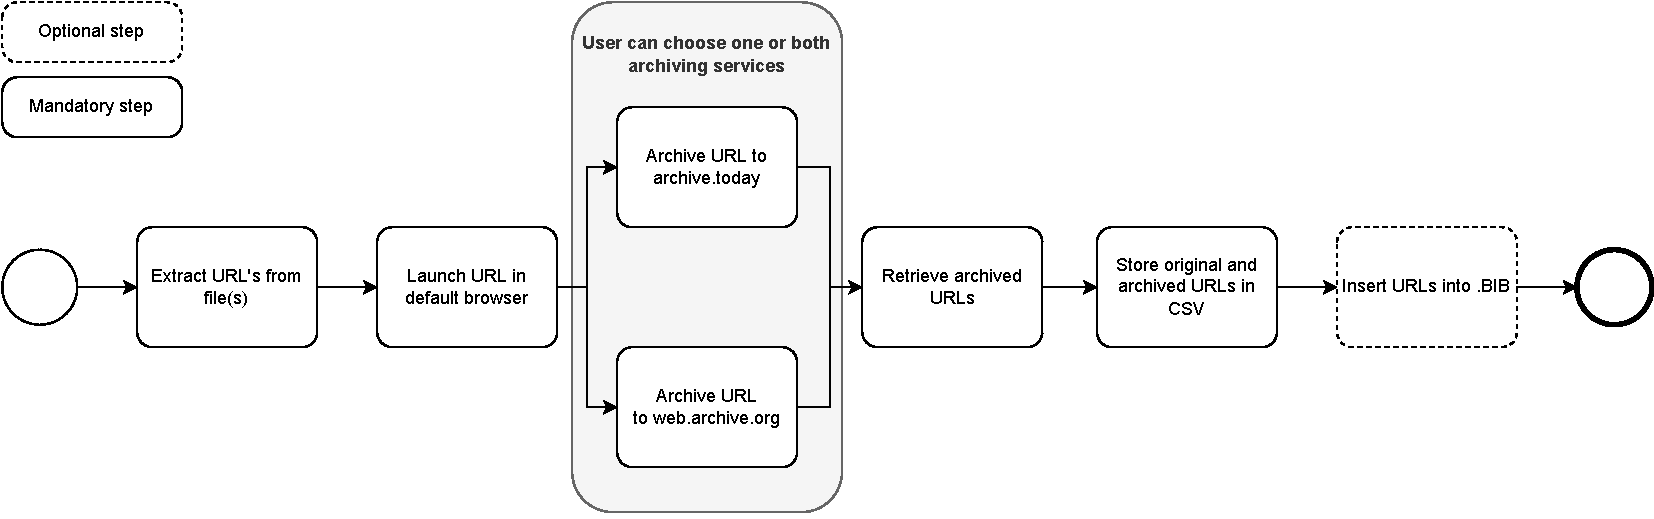
\includegraphics[width=1\textwidth]{pictures/process_model-simple}
    \end{frame}

    \begin{frame}{Technologies I}
        \begin{columns}
            \begin{column}{0.7\textwidth}
                \textbf{Core Technologies}
                \begin{itemize}
                    \item \textbf{Java}: The primary programming language for our application.
                    \item \textbf{LaTeX}: Used for documentation and presentation.
                \end{itemize}

                \vspace{1em} % Space between core and supporting technologies

                \textbf{Supporting Technologies}
                \begin{itemize}
                    \item \textbf{JUnit 5}: Utilized for unit testing.
                    \item \textbf{PDFTextStripper (PDFBox library)}: Used for extracting text from PDF documents.
                    \item \textbf{Selenium}: Web automation tool used for tasks like inputting URLs, handling captchas, and retrieving archived URLs due to the absence of an official API from archive.today.
                    \item \textbf{Maven}: Essential for compilation, dependency management, and building the project.
                \end{itemize}
            \end{column}

            \begin{column}{0.3\textwidth}
                
\includegraphics[height=0.5cm]{pictures/Java-Logo}
                \vspace{1em}
                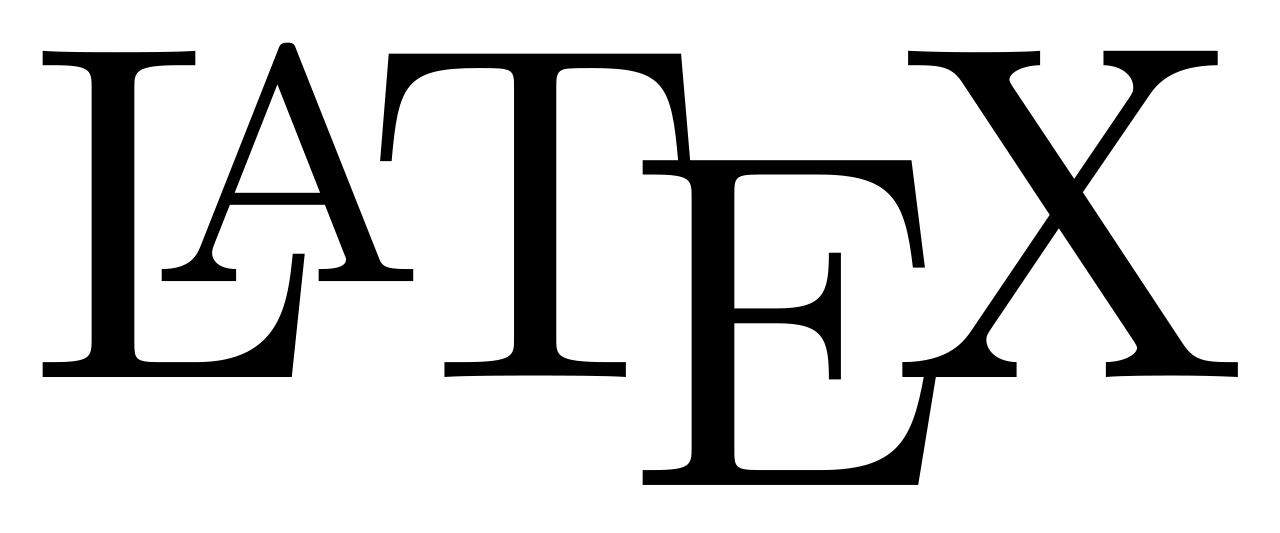
\includegraphics[height=0.5cm]{pictures/LaTeX_logo}
                \vspace{1em}
                
\includegraphics[height=0.5cm]{pictures/JUnit_5_Logo}
                \vspace{1em}
                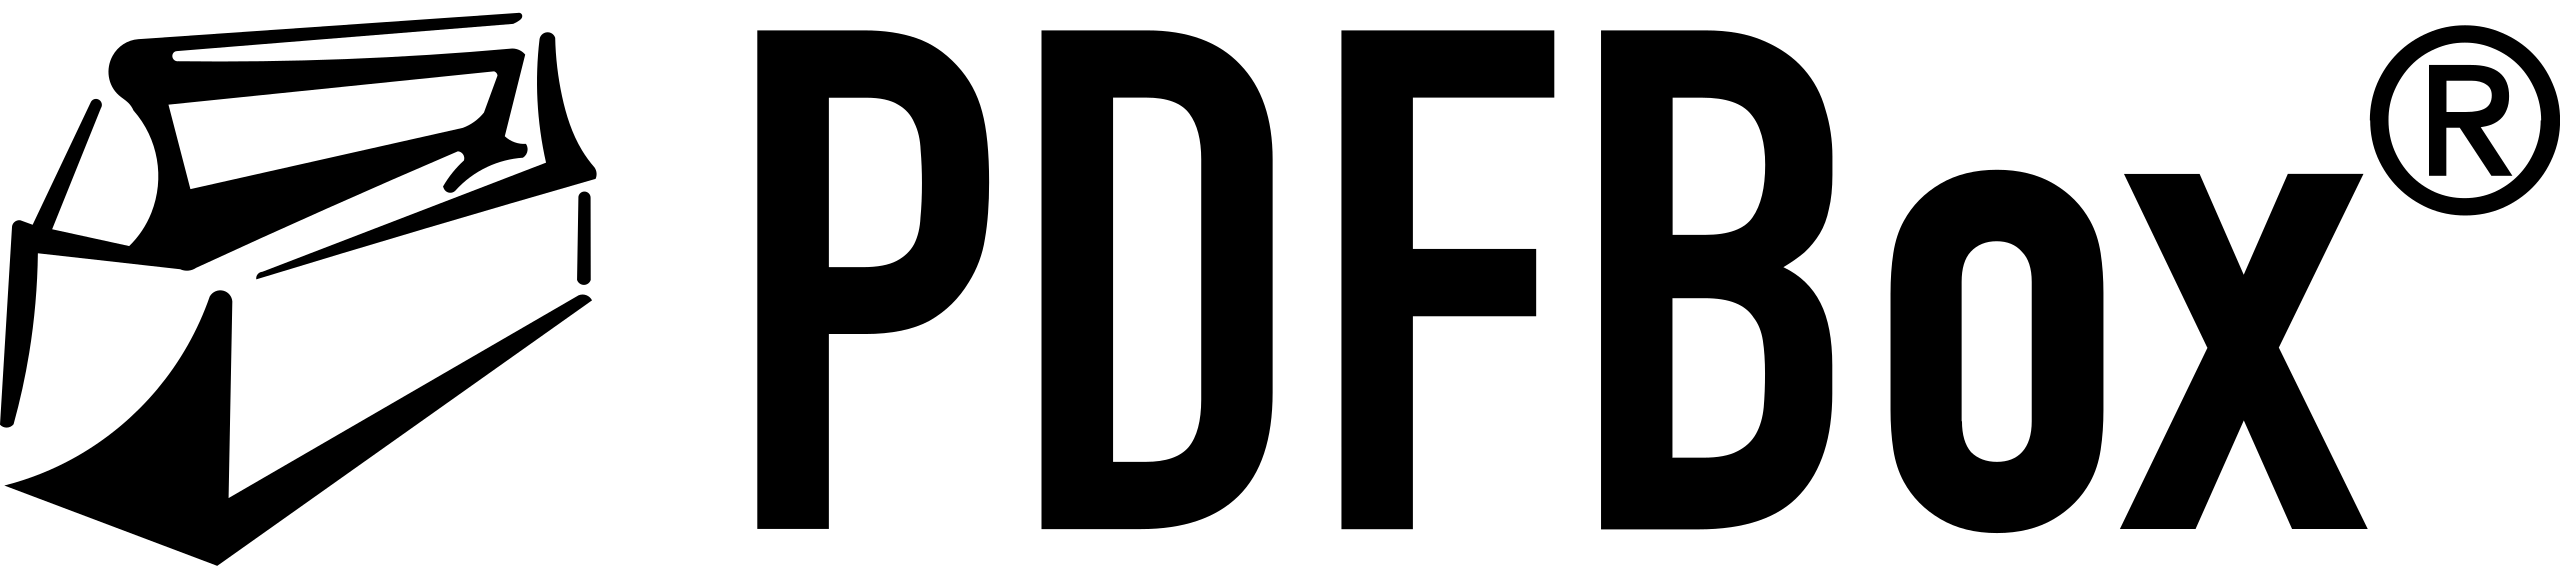
\includegraphics[height=0.5cm]{pictures/Apache_PDFBox_logo}
                \vspace{1em}
                
\includegraphics[height=0.5cm]{pictures/Selenium_logo}
                \vspace{1em}
                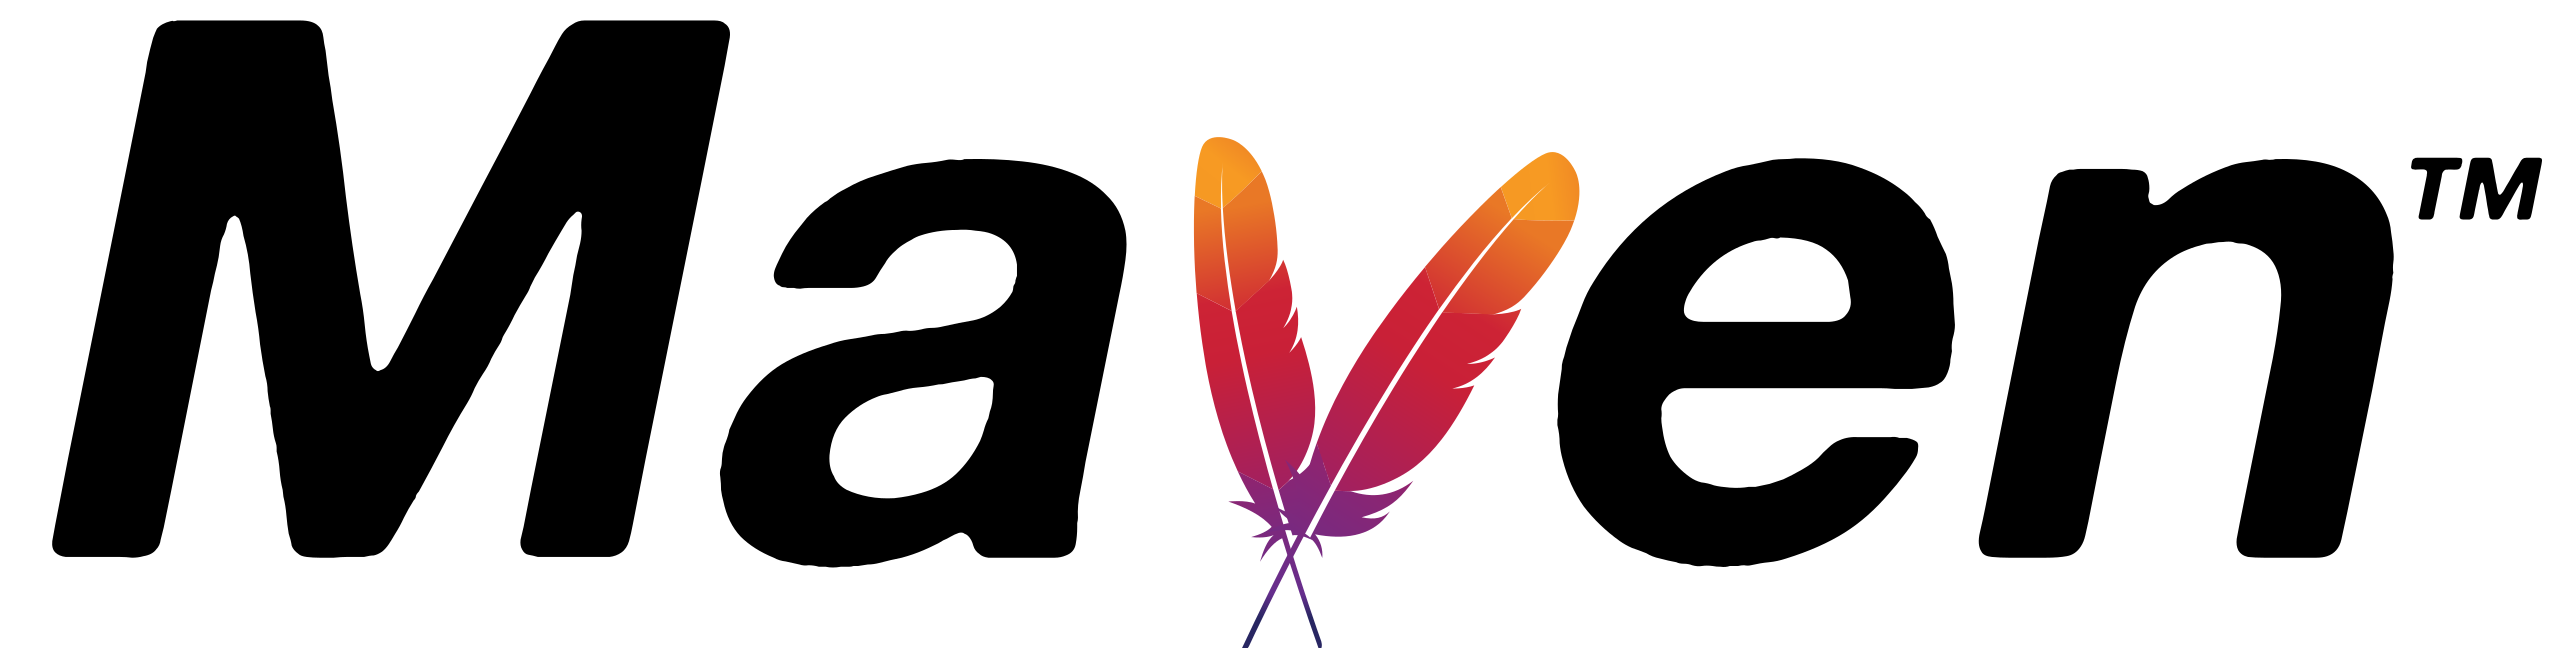
\includegraphics[height=0.5cm]{pictures/Apache_Maven_logo}
            \end{column}
        \end{columns}
    \end{frame}

    \begin{frame}{Technologies II}
        \begin{columns}
            \begin{column}{0.7\textwidth}
                \textbf{Archiving Services}
                \begin{itemize}
                    \item \textbf{Wayback Machine}: One of the services used by the URL-Archiver to archive URL's.
                    \item \textbf{Archive.today}: One of the services used by the URL-Archiver to archive URL's.
                \end{itemize}
            \end{column}
            \begin{column}{0.3\textwidth}
                
\includegraphics[height=1cm]{pictures/Wayback_Machine_logo}
                \vspace{1em}
                
\includegraphics[height=1cm]{pictures/archive_today_logo}
            \end{column}
        \end{columns}
    \end{frame}

    \begin{frame}{etc.}
        \framesubtitle{}
    \end{frame}
    %-------------------------------%

    % Chapter two "Project Management with SCRUM"


    \section{Project Management with SCRUM}
    \setbeamertemplate{section page}[BFH-ruled]
    \frame{\sectionpage}

    \begin{frame}{Scrum-Rollen}
        \framesubtitle{}
    \end{frame}

    \begin{frame}{Sprintziele}
        \framesubtitle{}
    \end{frame}

    \begin{frame}{Anforderungen}
        \framesubtitle{}
    \end{frame}

    \begin{frame}{Scrum Adaptionen}
        \framesubtitle{}
    \end{frame}

    \begin{frame}{etc.}
        \framesubtitle{}
    \end{frame}
    %-------------------------------%

    \begin{frame}{Blocks}
        \begin{block}{Block with a title}
            Content.
        \end{block}
        \begin{block}{}
            Without title
        \end{block}
    \end{frame}

    \begin{frame}{Block types}
        \begin{exampleblock}{Exampleblock}
            Content.
        \end{exampleblock}
        \begin{alertblock}{Alertblock}
            Content.
        \end{alertblock}
        \begin{example}[Example environment]
            Content.
        \end{example}
    \end{frame}


    \section{section pages}
%These can be automaticlly called by using \AtBeginSection{\sectionpage}

    \setbeamertemplate{section page}[BFH-ruled]
    \frame{\sectionpage}

%Change base color scheme (option can be added)

    %\setbeamercolor{BFH}{parent=BFH-Orange}

    %\frame{\sectionpage}

    %\setbeamertemplate{section page}[BFH]

    %\frame{\sectionpage}

\end{document}

